\documentclass{beamer}

\usetheme{CambridgeUS}

\usepackage{hyperref}
\usepackage{verbatim}

\title{Predicting Country GDP}
\subtitle{Using World Bank Development Indicators}
\date{\today}
\subject{Statistics}

\author{K.~Chen\inst{1} \and V.~Sharma\inst{1} \and JL.~Etienne\inst{1}}

\institute[Williams College] 
{
  \inst{1}
  Statistics 202 \\
  Williams College
}

\date{\today}

% Use for TOC at subsection start:
% \AtBeginSubsection[] { \begin{frame}<beamer>{Outline} \tableofcontents[currentsection,currentsubsection] \end{frame} }


\hypersetup{
    bookmarks=true,         % show bookmarks bar?
    unicode=false,          % non-Latin characters in Acrobat’s bookmarks
    pdftoolbar=true,        % show Acrobat’s toolbar?
    pdfmenubar=true,        % show Acrobat’s menu?
    pdffitwindow=false,     % window fit to page when opened
    pdfstartview={FitH},    % fits the width of the page to the window
    pdftitle={My title},    % title
    pdfauthor={Author},     % author
    pdfsubject={Subject},   % subject of the document
    pdfcreator={Creator},   % creator of the document
    pdfproducer={Producer}, % producer of the document
    pdfkeywords={keyword1} {key2} {key3}, % list of keywords
    pdfnewwindow=true,      % links in new window
    colorlinks=true,       % false: boxed links; true: colored links
    linkcolor=red,          % color of internal links (change box color with linkbordercolor)
    citecolor=green,        % color of links to bibliography
    filecolor=magenta,      % color of file links
    urlcolor=cyan           % color of external links
}

\begin{document}

\begin{frame}
\titlepage
\end{frame}

\begin{frame}{Outline}
\tableofcontents%[pausesections]
\end{frame}


% % % % % % % % % % % % % % % % % % % %
% % % % % % % % % % % % % % % % % % % %
% % % % % % % % % % % % % % % % % % % %
\section{Research Question}

%RESPONSE
\subsection{Response of Interest}
\begin{frame}{Response of Interest}
\begin{itemize}
\item What makes a country rich?
\item Two metrics for wealth:
	\begin{itemize}
	\item GDP
	\item GDP per capita
	\end{itemize}
\item Compare Japan and China (in 2012 USD)
\begin{table}
    \begin{tabular}{| l | l | l |} \hline
    ~     & GDP (in trillions) & GDP per capita (in thousands) \\ \hline
    China & 8.2                            & 6                                         \\ \hline
    Japan & 6                              & 46                                        \\ \hline
    \end{tabular}
\end{table}
\end{itemize}
\end{frame}



%DATA
\subsection{Data Overview}
\begin{frame}{Downloading the Data}
\begin{itemize}
	\item Collected from \href{http://data.worldbank.org/indicator}{The World Bank} 
	\item All countries -- Afghanistan to Zimbabwe
	\item Only two years -- 1980, 2008
		\begin{itemize}
	    \item \emph{time series} problems, e.g. autocorrelation
		\end{itemize}
\end{itemize}
\end{frame}

\begin{frame}{Long to Wide Format}
\begin{itemize}
	\item Use the {\tt reshape} package
	\item \emph{Long} format --- what we downloaded \\
		\begin{table}
			\begin{tabular}{ | l | l | l | } \hline
			Country		& Variable		& Value \\ \hline
			Afghanistan	& GDP1980		& 2.4   \\ \hline
			Afghanistan	& GDP2008  		& 2.7   \\ \hline
			Afghanistan	& CO$_2$1980  	& 4.6   \\ \hline
			Afghanistan	& CO$_2$2008  	& 5.6   \\ \hline
			\end{tabular}
		\end{table}
		
	\item \emph{Wide} format --- what we want \\
		\begin{table}
			\begin{tabular}{| l || l | l | l | l |} \hline
			Country		& GDP1980	& GDP2008	& CO$_2$1980	& CO$_2$2008 \\ \hline
			Afghanistan	& 2.4			& 2.7			& 4.6				& 5.6 \\ \hline
%			Albania		& 4.3			& 4.6			& 3.2				& 4.2 \\ \hline
			\end{tabular}
		\end{table}
\end{itemize}
\end{frame}

\begin{frame}{Parcelling Data into Frames}{Frame per Year}
\begin{itemize}
	\item What we have: \\
		\begin{table}
			\begin{tabular}{| l || l | l | l | l |} \hline
			Country		& GDP1980	& GDP2008	& CO$_2$1980	& CO$_2$2008 \\ \hline
			Afghanistan	& 2.4			& 2.7			& 4.6				& 5.6 \\ \hline
%			Albania		& 4.3			& 4.6			& 3.2				& 4.2 \\ \hline
			\end{tabular}
		\end{table}
		
	\item What we want (for each year): \\
		\begin{table}
			\begin{tabular}{ | l || l | l | } \hline
			Country     & GDP & CO2 \\ \hline
			Afghanistan & 2.4 & 4.6 \\ \hline
			\end{tabular}
		\end{table}
\end{itemize}
\end{frame}

\begin{frame}{Over 1300 Indicators}
\begin{itemize}
	\item Education -- literacy rates, public spending\dots
	\item Environment -- electricity access, CO2 emissions, water pollution\dots
	\item Economic Policy \& Debt
	\item Finance
	\item Health -- immunization, fertility, mortality, HIV, malnutrition\dots
	\item Infrastructure -- Internet/cell users, paved roads, rail lines\dots
	\item Labor -- unemployment
	\item Poverty
	\item Trade -- imports, exports
\end{itemize}
\end{frame}



%PREDICTORS
\subsection{Predictors of Interest}

% RURAL PREDICTOR
\subsubsection{Rural Population}

\begin{frame}{Rural Population}

\begin{columns}
  \begin{column}{0.5\textwidth}
    \begin{itemize}
        \item wellbeing indicator
        \item what percentage of rural population has access to clean water?
        \begin{figure}
	\centering
	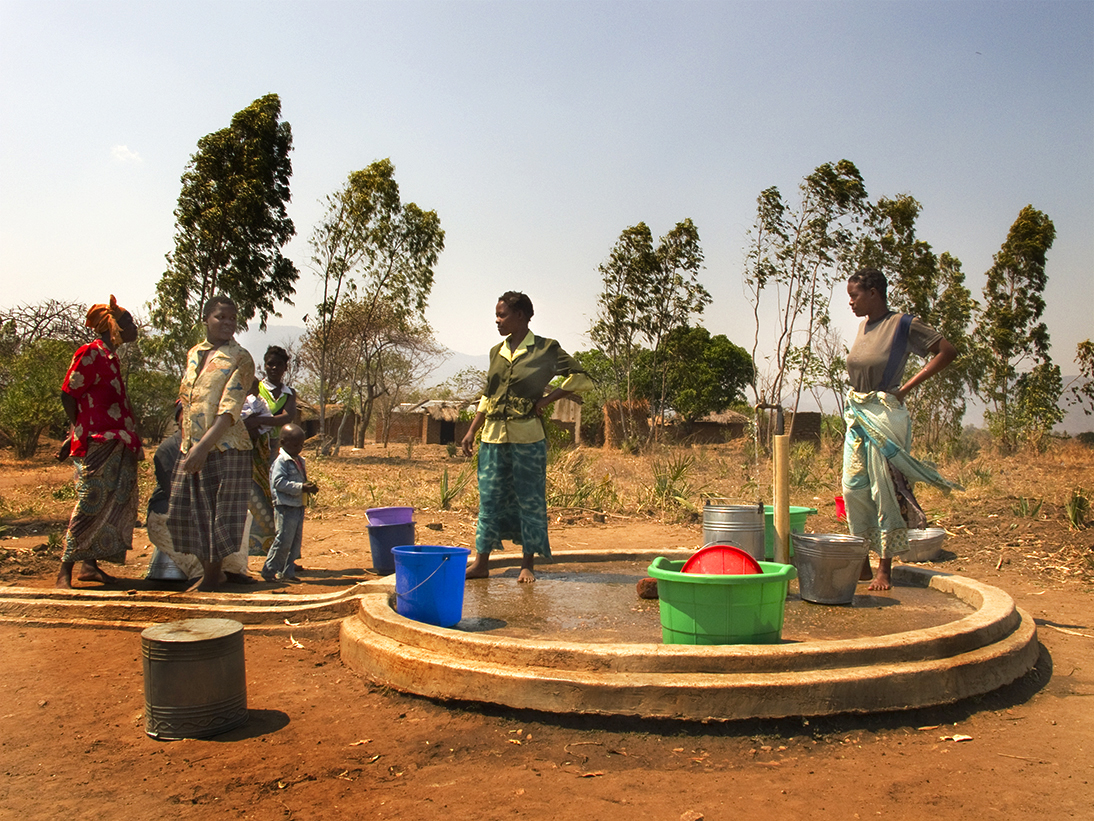
\includegraphics[scale=0.12]{images/malawi_rural_water.jpg}
	\caption{Rural water source in Malawi}
	\end{figure}
    \end{itemize}
  \end{column}

  \begin{column}{0.5\textwidth}
     \begin{itemize}
        \item structural indicator
        \item what percentage of country's population is rural?
        \begin{figure}
	\centering
	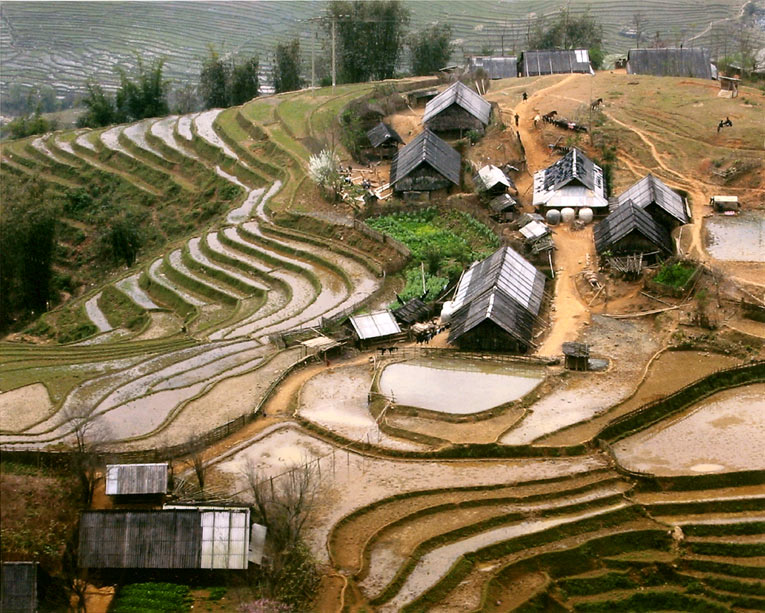
\includegraphics[scale=0.15]{images/sapa_vietnam_2003.jpg}
	\caption{Sapa, Vietnam 2003}
	\end{figure}
     \end{itemize}
  \end{column}
\end{columns}

\end{frame}

% CLIMATE PREDICTOR
\subsubsection{Climate Change}
\begin{frame}{Climate Change}

\begin{columns}
  \begin{column}{0.5\textwidth}
    \begin{itemize}
        \item electricity consumption
	        	\begin{figure}
		\centering
		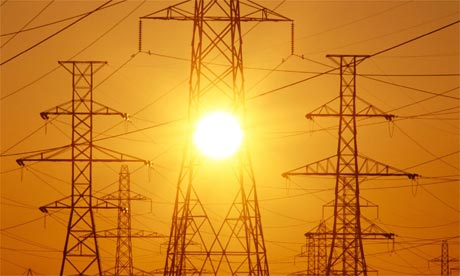
\includegraphics[scale=0.25]{images/electricity_consumption.jpg}
		\end{figure}
	\item pollution
		\begin{figure}
		\centering
		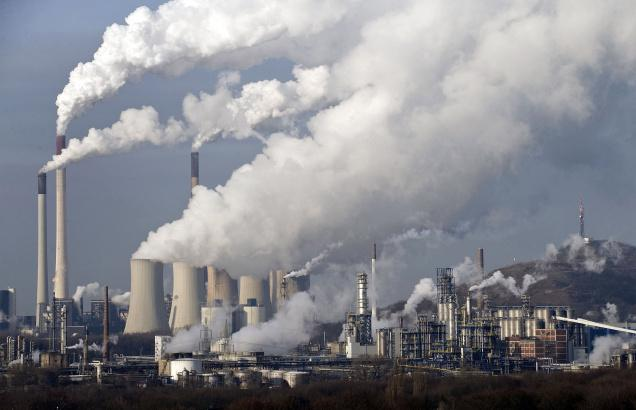
\includegraphics[scale=0.2]{images/pollution.jpg}
		\end{figure}
    \end{itemize}
  \end{column}

  \begin{column}{0.5\textwidth}
     \begin{itemize}
	\item paved roads
		\begin{figure}
		\centering
		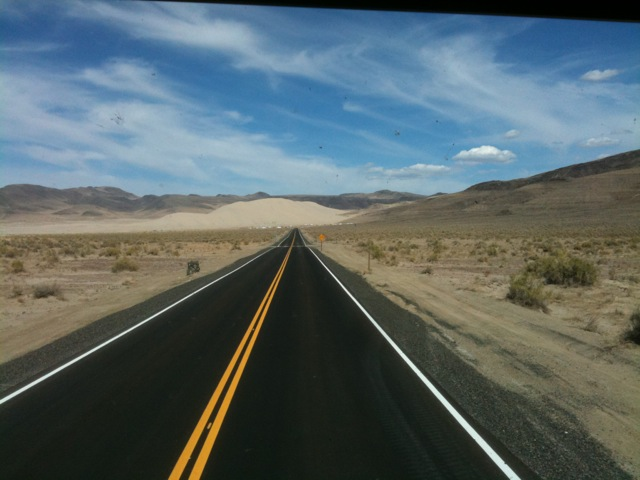
\includegraphics[scale=0.2]{images/paved_road.jpg}
		\end{figure}
     \end{itemize}
  \end{column}
\end{columns}
\end{frame}


% SOCIAL DEVELOPMENT PREDICTOR
\subsubsection{Social Development}

\begin{frame}{Social Development}
\begin{columns}
  \begin{column}{0.5\textwidth}
    \begin{itemize}
        \item life expectancy
        \item child labor
        \begin{figure}
	\centering
	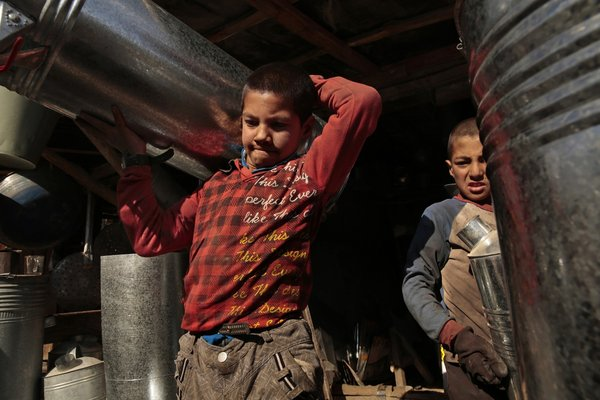
\includegraphics[scale=0.55]{images/child_labor.jpeg}
	\caption{Child labor in metal shop, Kabul. LATimes.}
	\end{figure}
    \end{itemize}
  \end{column}

  \begin{column}{0.5\textwidth}
     \begin{itemize}
        \item literacy rates
        \item refugee population
        \begin{figure}
	\centering
	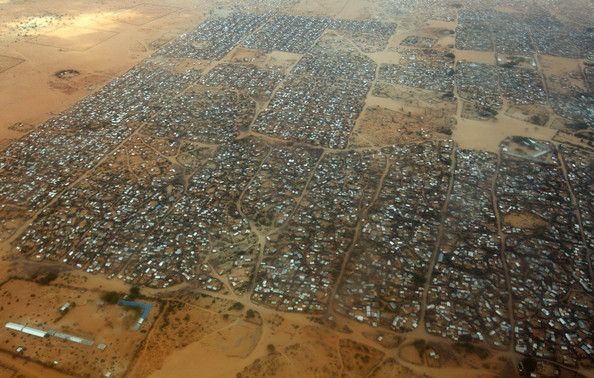
\includegraphics[scale=0.2]{images/refugee_camp.jpg}
	\caption{Aerial view of refugee camp in Dadaab, Kenya.}
	\end{figure}
     \end{itemize}
  \end{column}
\end{columns}
\end{frame}


% SCIENCE PREDICTOR
\subsubsection{Science}
\begin{frame}{Science Predictors}
\begin{itemize}
\item high tech exports
\item science journals
\item research and development

\begin{figure}
	\centering
	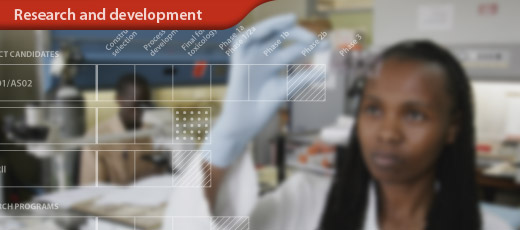
\includegraphics[scale=0.5]{images/research_and_development.jpg}
\end{figure}

\end{itemize}
\end{frame}

% TODO add LABOR PREDICTOR frame
% unemployment, service/industry/agriculture sector male-female composition


% % % % % % % % % % % % % % % % % % % %
% % % % % % % % % % % % % % % % % % % %
% % % % % % % % % % % % % % % % % % % %
\section{Exploratory Data Analysis}

% % % % % % % % % % % % % % % % % % % %
% % % % % % % % % % % % % % % % % % % %
% % % % % % % % % % % % % % % % % % % %
\section{Checking Model Conditions}

% % % % % % % % % % % % % % % % % % % %
% % % % % % % % % % % % % % % % % % % %
% % % % % % % % % % % % % % % % % % % %
\section{Final Model}

% % % % % % % % % % % % % % % % % % % %
% % % % % % % % % % % % % % % % % % % %
% % % % % % % % % % % % % % % % % % % %
\section{Conclusion}

% % % % % % % % % % % % % % % % % % % %
% % % % % % % % % % % % % % % % % % % %
% % % % % % % % % % % % % % % % % % % %
\section{Future Extensions}

\subsection{Stepwise Selection of Predictors}

\begin{frame}{The step function}
\begin{itemize}
\item Predictors selected automatically.
\item Yields a perfect model with an $R^2$ value $> 99.9$\%.
\item $\textrm{GDP per capita} = $
\end{itemize}
\end{frame}


\end{document}


